\chapter{DESAIN DAN IMPLEMENTASI}
\label{chap:desainimplementasi}

% Ubah bagian-bagian berikut dengan isi dari desain dan implementasi

Penelitian ini dilakukan sesuai dengan desain sistem yang telah disusun, yang melibatkan konseptualisasi infrastruktur dan perancangan blok-blok alur yang harus dijalankan. Setiap blok dalam desain sistem ini mencakup langkah-langkah implementasi yang dirancang secara teknis untuk mendukung visualisasi pembuluh darah secara menyeluruh. 

\section{3.1 Desain dan Deskripsi Sistem}

\begin{figure}[h!]
\centering
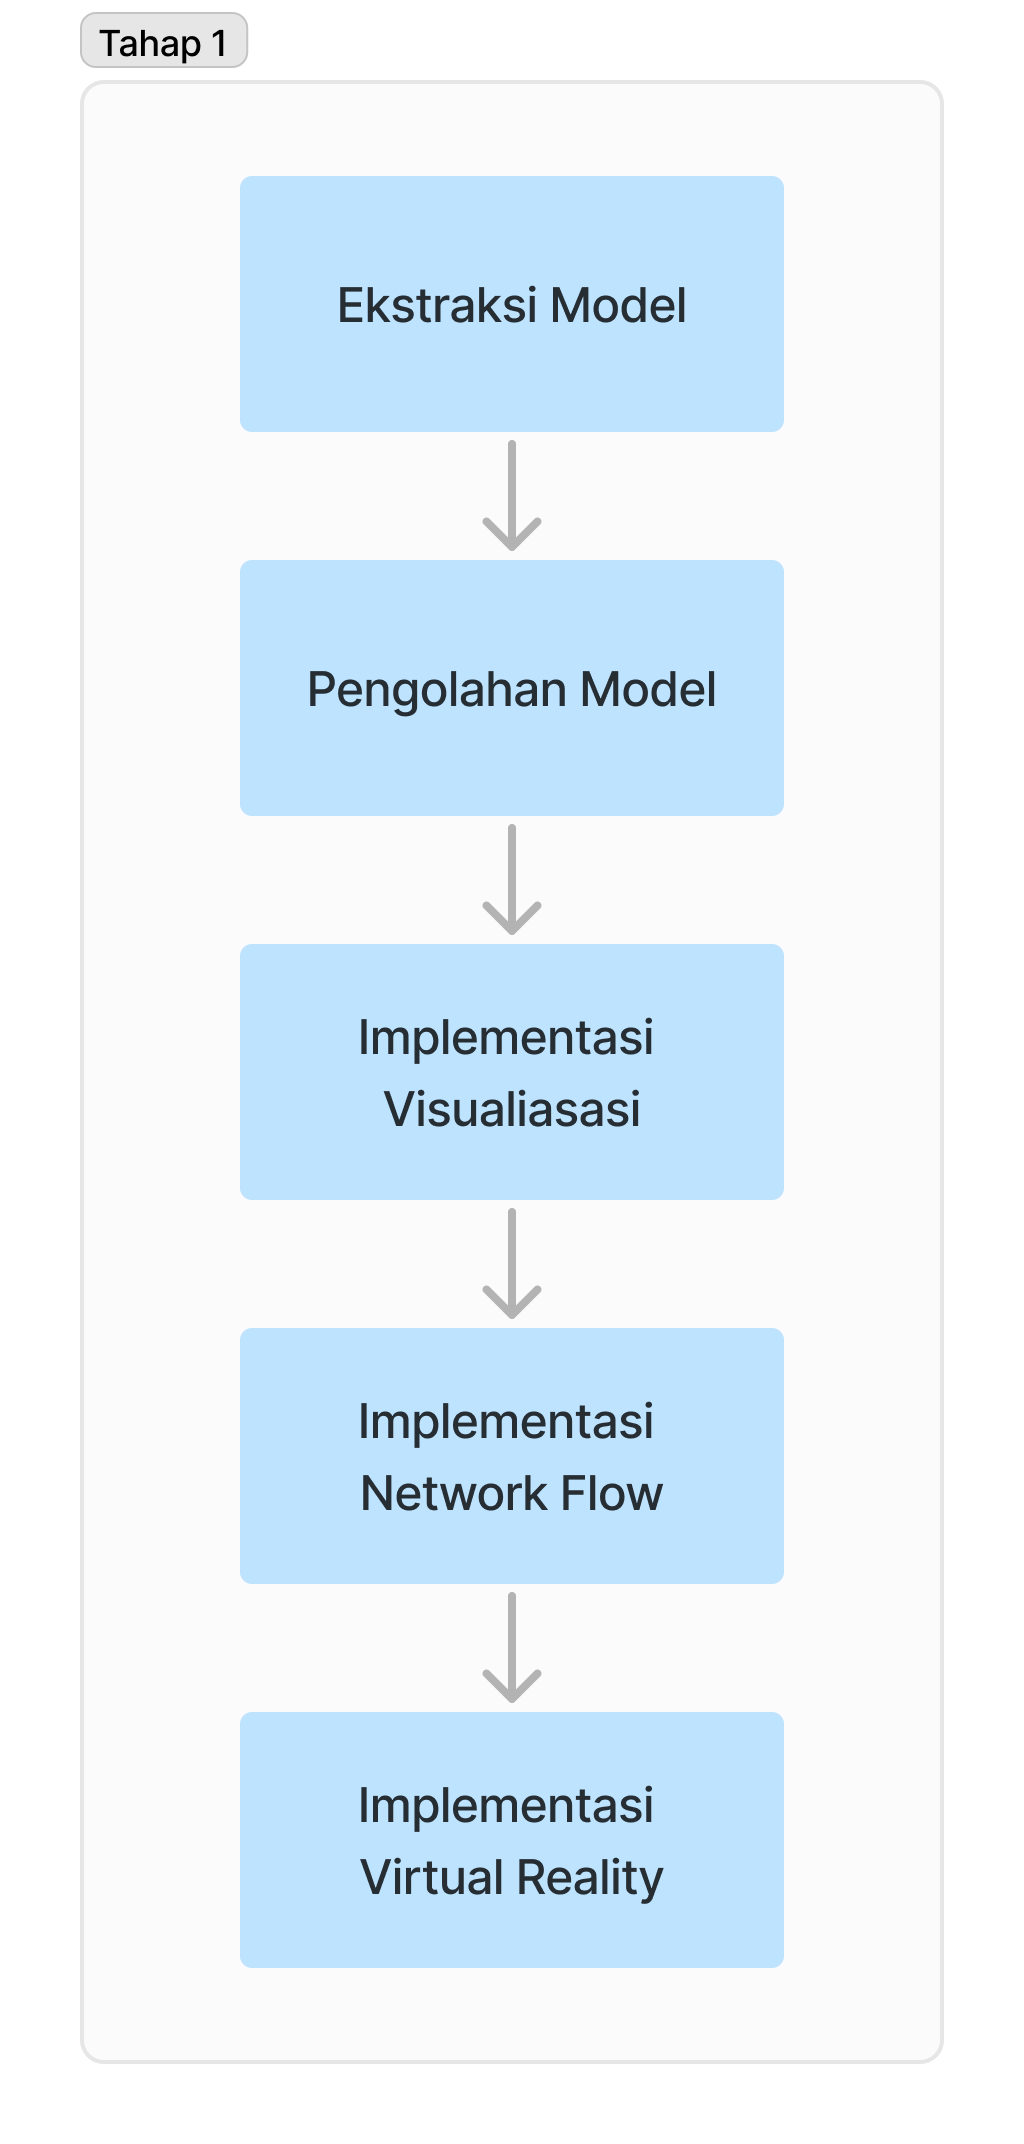
\includegraphics[width=0.4\textwidth]{gambar/Desain Implementasi 1.png}
\caption{Blok Diagram Sistem Visualisasi Pembuluh Darah}
\label{fig:flowchart}
\end{figure}

Pada Gamber \ref{fig:flowchart}, desain sistem visualisasi pembuluh darah dimulai dengan proses \textit{Ekstraksi Model}, dimana model didapatkan dari sumber penelitian terdahulu. dengan menggunakan tools Assets Studio pada precompiled unity game yang didapatkan dari penelitian sebelumnya, tentu dengan izin dari sang pemilik hak cipta.

Setelah tahap ekstraksi selesai, dilakukan proses \textit{Pengolahan Model}. Pada tahap ini, model pembuluh darah akan diekstrak dari model 3D manusia. model pembuluh darah akan dipotong berdasarkan alur pembuluh darah. selanjutnya akan diterapkan \emph{UV unwrapping} pada setiap potongan pembuluh darah. setelah model melewati semua tahapan tersebut, model akan di ekspor dalam fromat yang didukung oleh \emph{Unity Game Engine} 

Selanjutnya, model yang telah diproses akan masuk ke tahap \textit{Implementasi Visualisasi}. Pada tahap ini, model telah dimasukkan kedalam \emph{Unity Game Engine}, pada tahap ini pula akan dilakukan pembuatan Shader Graph untuk menvisualisasikan tekanan pada pembuluh darah, dan juga menvisualisasikan sumbatan yang terjadi pada pembuluh darah.

Tahap berikutnya adalah \textit{Implementasi Network Flow}, dimana dilakukan pembuatan graph masif dengan setiap komponen pembuluh darah akan mewakili \emph{edge} dan persimpangan antara pembuluh adarh akan mewakili \emph{vertex}. alghoritma \emph{Network Flow} akan diimplementasikan dengan menggunakan python FastAPI sebagai Backend yang akan dipanggil oleh APIService aplikasi.    

Tahap terakhir adalah \textit{Implementasi Virtual Reality (VR)}. Pada tahap ini, model pembuluh darah yang telah divisualisasikan dimasukkan ke dalam lingkungan realitas virtual. Implementasi VR ini memungkinkan pengguna untuk berinteraksi langsung dengan model pembuluh darah dalam ruang tiga dimensi yang imersif. Dengan teknologi VR, pengguna dapat mengeksplorasi model secara mendetail, baik untuk keperluan penelitian, edukasi, maupun diagnosa medis.

Dengan pendekatan yang sistematis dan terstruktur ini, sistem visualisasi pembuluh darah dapat diimplementasikan secara efisien, menghasilkan model yang tidak hanya akurat tetapi juga mudah untuk digunakan dalam berbagai aplikasi medis.

\section{Implementasi Alat}
\label{sec:implementasi alat}

\subsection{Ekstraksi Model}

